\label{s:methods}
\subsection*{Feasible activation set}
For ease of presentation and visualization,  first describe this novel approach in a  3-muscle system acting on a  rotational joint as shown in Fig. \ref{fig:schematic_arm}, and then demonstrate its utility and in a realistic model of the human index finger with 7 muscles. 

Consider a tendon-driven limb with $n$ muscles. As described in \cite{Kuo1993Human, Chao1978Graphical,spoor1983balancing,Valero-Cuevas2009mathematical, valero-cuevas2015neuromechanics}, we can describe  the neural command to a muscle is a positive value of activation $0 \leq a \leq 1$.  If there are $n$ independently controlled  muscles,  the set of all feasible neural commands  is the positive unit $n$-cube, and the coordination patters in the vector $\textbf{a} \in \mathbb{R}^n$ as explained in \cite{Valero-Cuevas2009mathematical, valero-cuevas2015fundamentals}. Moreover, when  task constraints are introduced, only those points within the $n$-cube that meet those constraints are allowable. In the context of producing a vector of static force with the endpoint of the limb in a give posture, the constraints that define that task (i.e., the direction and magnitude of the force vector at the endpoint) are linear equations.  Each constraint equation defines a hyper-plane of dimension $n-1$. The \emph{feasible activation set} of the task, if it exists,  is formed by the intersection of the $n$-cube and the hyperplanes.
Thus if the limb can meet all constraint equations, described as the rows of matrix $A$, the feasible activation set is given by the convex polytope $P$ containing all $\textbf{a} \in \mathbb{R}^n$, that satisfy
\begin{align}
\label{eq:constraints}
		\textbf{f} = A\textbf{a}, \textbf{a} \in [0,1]^n
\end{align}
where $\textbf{f} \in \mathbb{R}^m$ is the desired endpoint force vector.
The dimensionality of output, $m$, is  at most 6-dimensional (i.e., 3 forces and 3 torques) depending on the number of kinematic degrees of freedom of the limb, and usually $m < n$  because  limbs have numerous  muscles \cite{Valero-cuevas2015fundamentals}. Thus, if $\textbf{f}$ is a feasible  output, the feasible activation set $P$ is a $(n-m)$-dimensional convex polytope embedded into the $n$-cube.
\begin{figure}[h]
  \label{fig:schematic_arm}
  \centering
  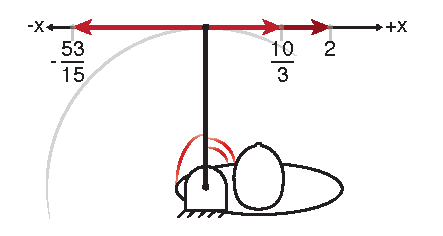
\includegraphics{figs/schematic_arm_1D.pdf}
  \caption{One imagined visualization of the fabricated tendon driven system, with 3 generators.}
\end{figure}
In particular, consider the simple case of $A  \in \mathbb{R}^{1 \times 3}$  illustrated in Fig. \ref{fig:schematic_arm}, where the task is to produce a 1 Newton force in the rightward $x$ direction with the endpoint of a rigid link that is hinged to lie in the plane, and is actuated by 3 muscles.
The set of feasible activations is given by the shaded convex polygon in Fig. \ref{fig:polygon_slice_solution_space}. This is because there are three independently controlled muscles meeting one linear   constraint. Thus $P$ is of dimension $(3-1) = 2$. In this case, we define a sample constraint equation 

\begin{align}
\label{eq:constraint}
\begin{split}
	&+1 = \frac{10}{3}a_1 - \frac{53}{15}a_2 + 2a_3 \\
&a_1, a_2, a_3 \in [0,1],
\end{split}
\end{align}
that represents how the sum of forces that each muscle produces at the endpoint must add to $+1$. The coefficients indicate the magnitude and direction of endpoint force each muscle produces.


\begin{figure}[t]
  \label{fig:polygon_slice_solution_space}
  \centering
  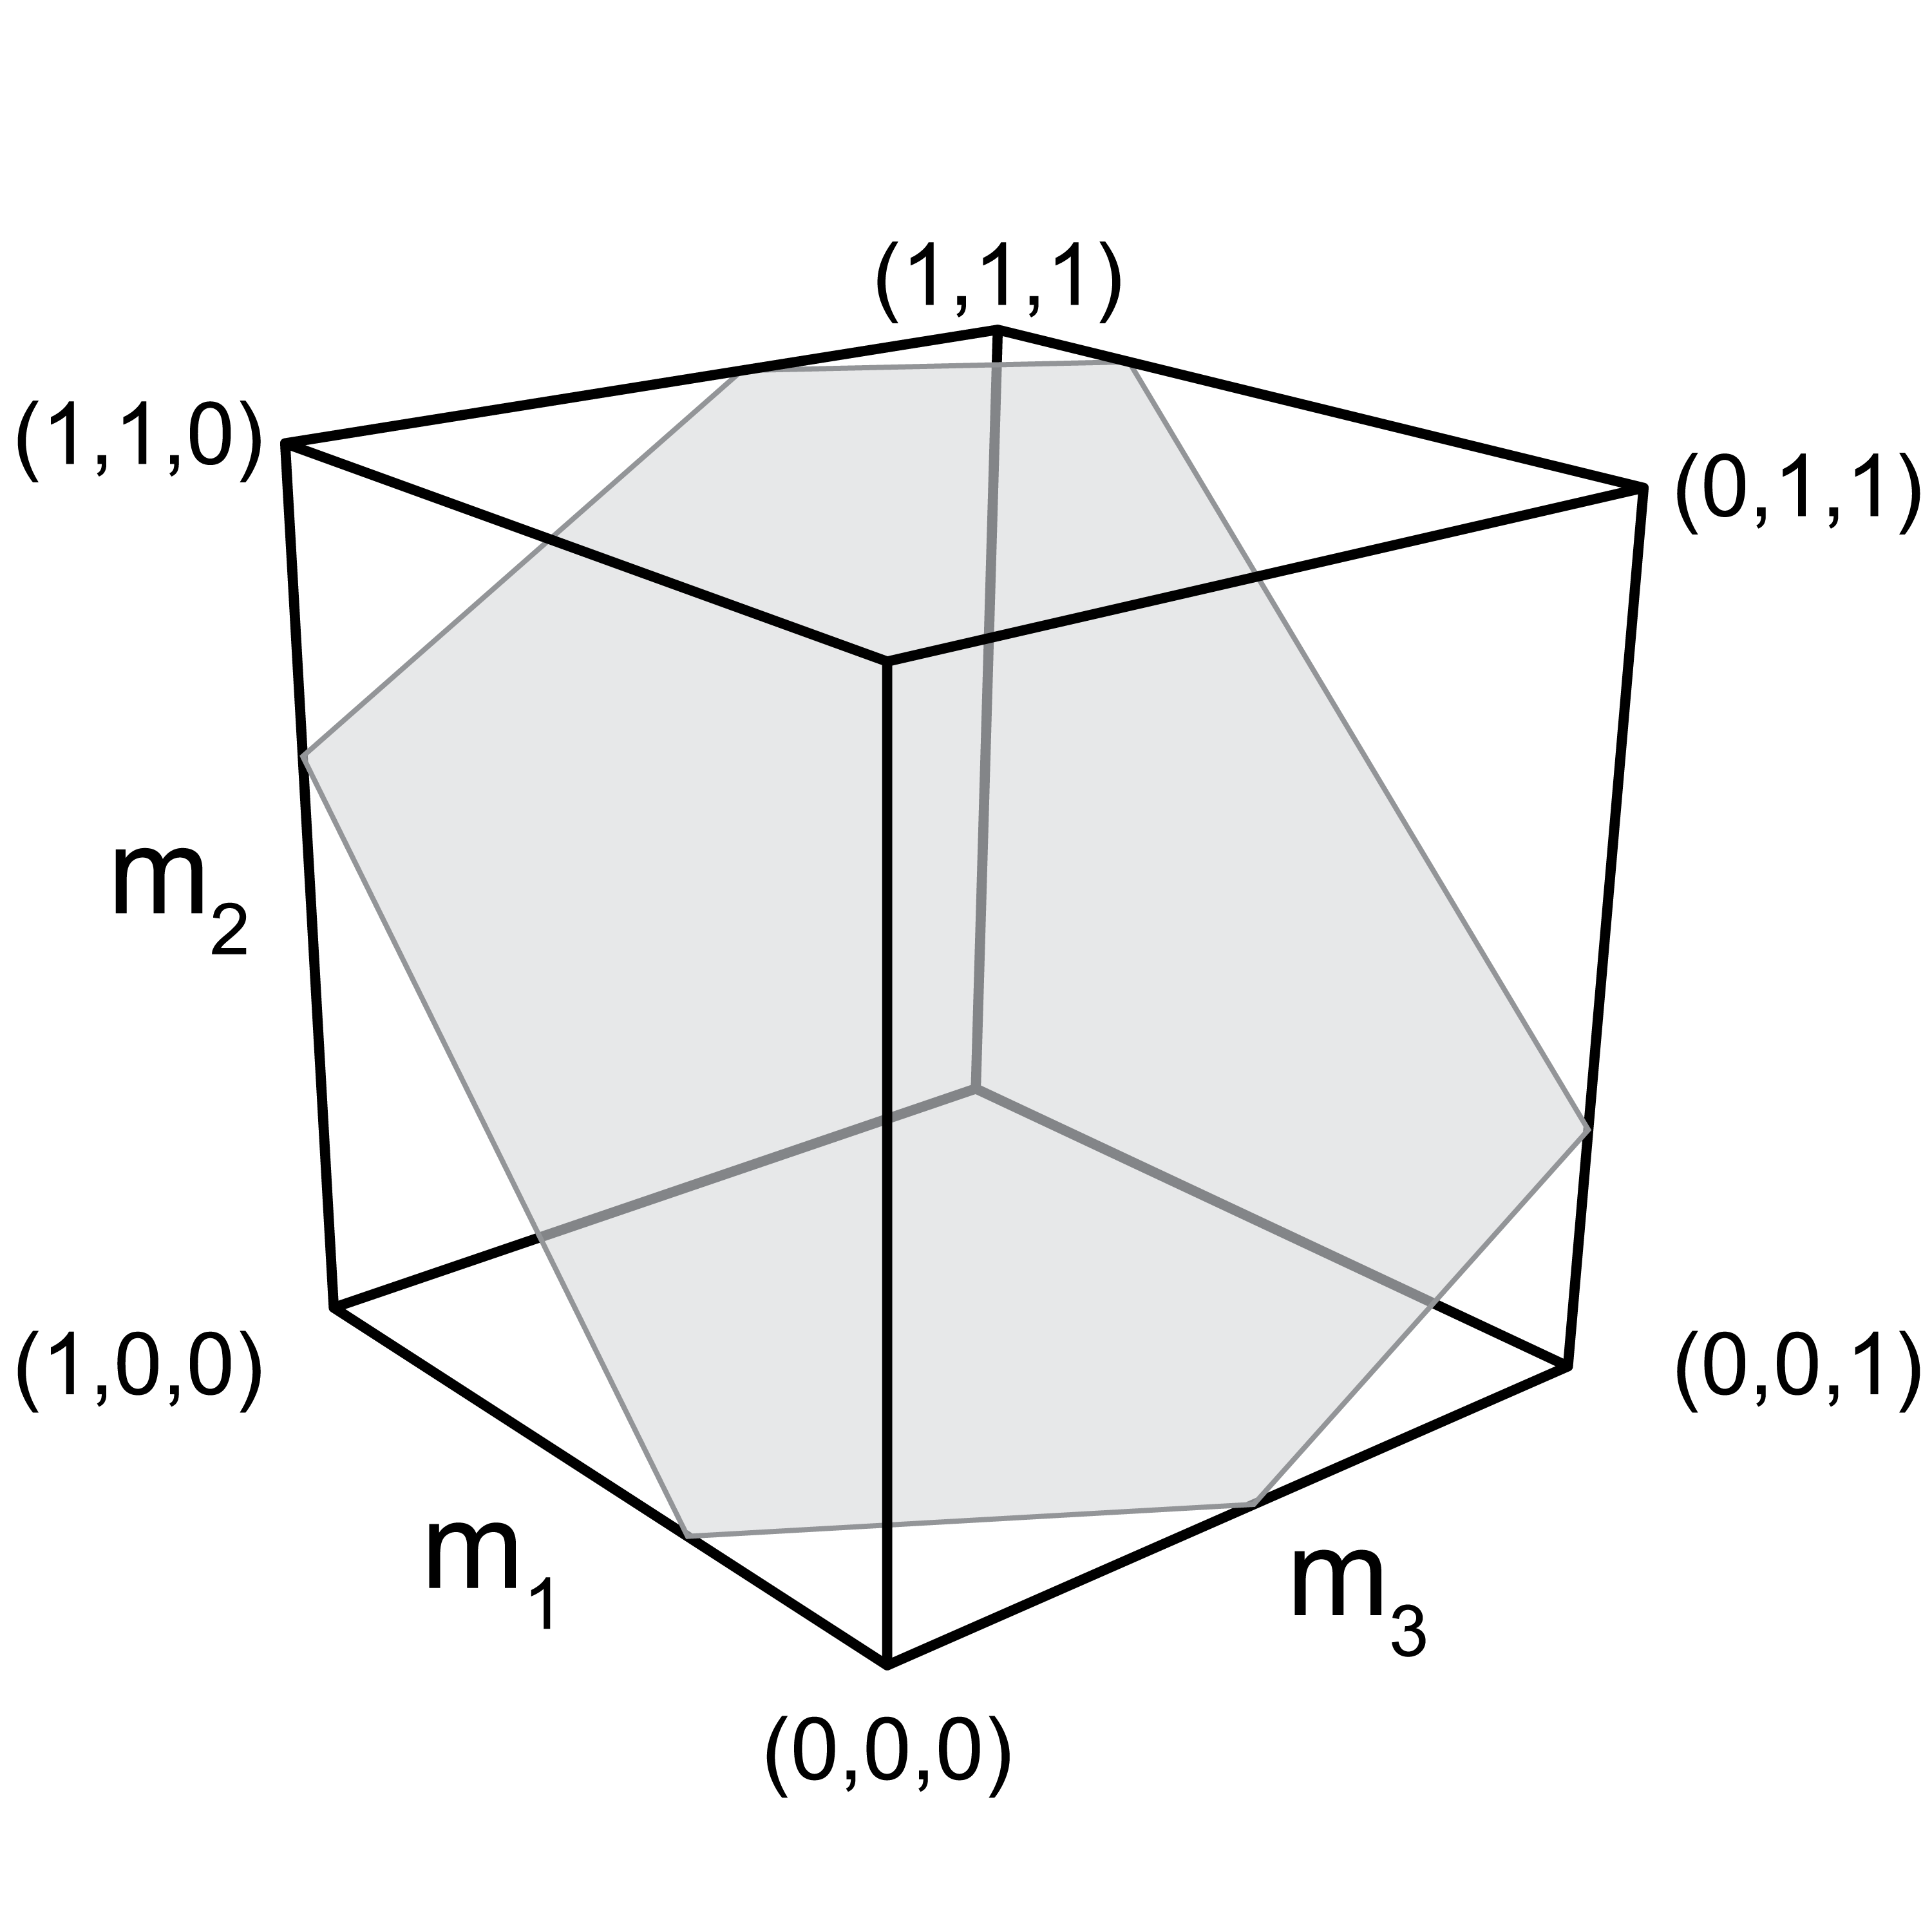
\includegraphics[width=0.25\textwidth]{sections/figs/feasibleactivation.png}
  \caption{The feasible activation set for a  three-muscle system meeting one functional constraint is a polygon in $\mathbb{R}^3$.} %Note that muscle activations are assumed to be bounded between $0$ and $1$.}
\end{figure}

\subsection*{The Hit-and-Run algorithm as a means to overcome difficulties in characterizing feasible activation sets  in higher dimensions}
\label{ss:hitrun}
We are interested in characterizing the qualities that define the muscle activation vectors $\textbf{a}$ that define $P$. But calculating the geometric properties of convex polytopes in high dimensions is computationally challenging. Take volume as an example, where the exact volume computations for polytopes is known to be $\#P$-hard \cite{Dyer}.
Thus available volume algorithms  can only handle polytopes embedded in small dimensions like 10 or slightly more \cite{Bueler2}.   Studying limbs in general, however, can require including  several dozen muscles, such as our studies of a 17-muscle human arm and a 31-muscle cat hindlimb model \cite{Valero-Cuevas2015high-dimensional}; and other limb models have over 40 muscles such as  \cite{arnold2010model, kutch2012challenges, hamner2010muscle, de2014human}.

Similar difficulties arise when computing the shape and aspect ratio of $P$ in high dimensions. We and others  have described $P$ by its bounding box  \cite{sohn2013cat_bounding_box,kutch2011muscle}, but  that  severely overestimates the shape and volumen of the feasible activation set as discussed in \cite{Valero-Cuevas2015high-dimensional}. Take Fig. \ref{fig:polygon_slice_solution_space} as an example, where the bounding box of the polygon has a volume---even though a plane has zero volume---, and can be almost as large as the positive unit cube itself. Similar problems arise in the interpretation of the inscribed and circumscribed ball. [or is it inscribing ball?]

We propose  describing the qualities that define the muscle activation vectors $\textbf{a}$ in the feasible activation set $P$ by the statistics, histograms, and point densities extracted by uniformly sampling the polytope. We used the Hit-and-Run method to sample  the convex polytope $P$ because it is known to converge to the uniform sampling across any convex body, called  $K$ in the general case \cite{smith1984efficient}.
It is a generalization of a discrete Markov chain, which recursively samples a sequence of points in $K$ as described below.
It is shown that after $\mathcal{O}^*(n^2R^2/r^2)$ steps, where $r$ and $R$ are the radii of the inscribed and circumscribed ball of $K$ respectively \cite{Dyer, Lovasz}, the Hit-and-Run algorithm has sampled a point uniformly-at-random (u.a.r.) from any starting point in $K$.[this last sentence is unclear. You cannot sample a point uniformly, you can only  sample uniformly from a range.... please clarify]
Unfortunately the hidden constant is large [what is the hidden constant? explain and provide a citation], which makes it practically infeasible to obtain the theoretical guarantee of convergence  with an u.a.r. walk.
Experimental results [give ref], however, suggest that a number of points linear with respect to the dimension suffices (as discussed in Section \ref{sec_lengthrun}).
[Move to appropriate place in the discussion: We chose Hit-and-run because of its easy structure and mixing guarantee; however, it would be interesting to compare Hit-and-Run with the Grid Walk, Ball walk, or other sampling paradigms \cite{Vempala}.]

The application of the Hit-and-Run method to $P$ is defined as follows (it works analogously for any convex body):

\begin{enumerate}
\item Find a starting point $\textbf{p}$ in $P$.
\item Generate a random direction $q$ (u.a.r.\ over all directions) from $\textbf{p}$ in $P$  (Fig. \ref{fig:hitruncube}a).
\item Find the two intersection points of the line given by the random direction $q$ with the boundary of the polytope (Fig. \ref{fig:hitruncube}b).
\item Choose a new point u.a.r. on the line segment between  the intersection points (Fig. \ref{fig:hitruncube}c). 
\item Repeat from $2.$ the above steps using the new point as the starting point, for $s$ iterations until the model is mixed as shown in Fig. \ref{fig:posthitrun_distribution}. [how do we say ``the model is mixed'' in English? Until convergence of the statistical properties of the samples points? Until convergence as per some convergence statistic?]
\end{enumerate}

\begin{figure}[h]
\centering
\includegraphics[width=0.5\textwidth,page=10]{sections/figs/HitandRunSchematics_all.pdf}
\caption{Graphical description of the Hit-and-Run algorithm.}
\label{fig:hitruncube}
\end{figure}

\begin{figure}[h]
\centering
\includegraphics[width=0.3\textwidth,page=9]{sections/figs/HitandRunSchematics_all.pdf}
\caption{Uniform distribution aross the feasible activation space.\ In the schematic arm example, the distribution is represented within a 2D plane.}
\label{fig:posthitrun_distribution}
\end{figure}

We describe the mathematical basis and full notes of our implementation in the appendix.

\subsection*{Realistic index finger model}
\label{ss:finger}
We  applied this methodology to our published model of an index finger for static fingertip force production\footnote{The model of the finger encapsulates the mechanics of static force production capabilities of the tendon-driven system $H=J^{-T}RF_o \in \mathbb{R}^{4 \times 7}$--- where $J$, $R$ and $F_0$ are the matrices of the Jacobian of the finger with 4 kinematic degrees of freedom, the moment arms of the tendons, and the strengths of the seven muscles, respectively \cite{Valero-Cuevas1998Large,Valero-cuevas2015fundamentals}}. It contains  four kinematic degrees of freedom (ad-abduction, flexion-extension at the metacarpophalangeal joint, and flexion-extension at the proximal and distal interphalangeal joints) and seven muscles  \cite{Valero-Cuevas1998Large}. The task we explored was producing a submaximal force in the `distal'  direction, shown  in Fig. \ref{fig:finger}, by combining this model with the constraints defining the direction of the force and the cancellation of endpoint torque. The finger posture was defined to be $0^\circ$  ad-abduction and $45^\circ$ flexion at the metacarpophalangeal joint, and $45^\circ$ and $10^\circ$ flexion, respectively, at the proximal and distal interphalangeal joints. For details on how create such models and apply task constraints see \cite{Valero-Cuevas1998Large,valero-cuevas2015fundamentals}.  This results in a model of the task where the resulted in a matrix $A \in \mathbb{R}^{4 \times 7}$, where $\textbf{a} \in \mathbb{R}^7$. Each row is a constraint: The first two constraints define the up-down and  left-right directions of the fingertip force vector, and the third equation sets the torque at the fingertip to zero. The fourth constraint sets the magnitude of the distal force to a particular value. Thus the task has a 4-dimensional null space. Thus the feasible activation set $P$ is a 4-dimensional convex polytope embedded in 7-dimensional muscle activation space.

[[[there is a problem in how things were written: The A matrix is one that includes the constraints. it is not the unconstrained model. Thus, A is not the model. A is the  set of constraints based on the model and the task constraints---the null space of the task. This resulted in a matrix $A \in \mathbb{R}^{4 \times 7}$, where $\textbf{a} \in \mathbb{R}^7$. ]]]


\begin{figure}[ht]
  \centering
  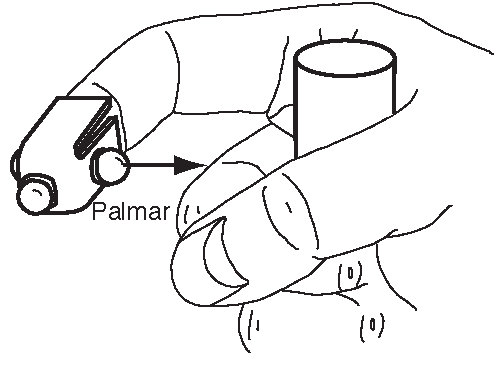
\includegraphics[]{sections/figs/finger.pdf}
  \caption{The index finger model simulated force production in the distal direction. Adapted from \cite{Valero-Cuevas1998Large}.}
  \label{fig:finger}
\end{figure}


\subsection*{Histograms of points samples from the feasible activation set}
The set of points sampled from the convex polytope can be visualized by the muscle-by-muscle histograms.  This is particularly  helpful to  visualize the relative number of solutions (i.e., density of solutions) that required a particular level of activate from a particular muscle within its native range of $[0,1]$. In addition, the upper and lower bounds of the histograms show the length of the bounding box of the polytope in every dimension. 

\subsection*{Parallel coordinates visualization}
A common way to visualize high-dimensional coordinate data is using parallel coordinates, which has been used in biomechanical studies \cite{bachynskyi2013biomechanical, krekel2010visual}.
For the results of the simple example shown in Fig. \ref{fig:posthitrun_distribution}, we begin by drawing $n$ parallel lines for each of the $n$ (i.e., 3) muscles.
With the axis labels of the line set between 0 and 1, each point is then represented by connecting their coordinates by $n-1$ lines as shown in Fig. \ref{fig:points_to_parcoords_mapping}a and \ref{fig:points_to_parcoords_mapping}b. 


\begin{figure}[ht]
  \centering
  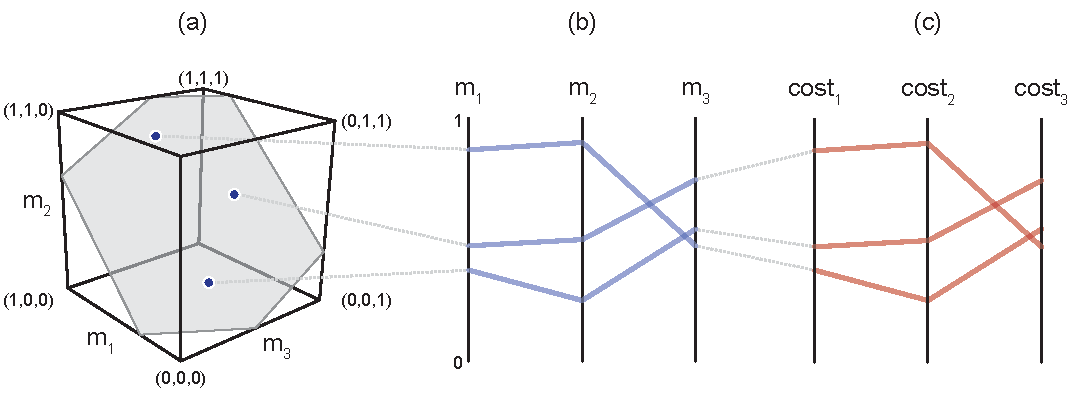
\includegraphics[width=1.0\textwidth]{sections/figs/3d_points_to_parcoords.pdf}
  \caption{Schematic mapping between 3D points (a), activations in parallel coordinate format (b), and the associated costs of each activation (c).
Activations in in the parallel coordinate format are set between $0 and 1$, and cost bounds are normalized to the range of the observed cost.}
  \label{fig:points_to_parcoords_mapping}
\end{figure}


Applying this visual interface to the index finger model  we can, for example,  restrict the range of muscle activation of one or multiple muscles to any desired interval to explore the associated activation levels of the remaining muscles as shown in Fig. \ref{fig:parcoord_full} and \ref{fig:parcoords}.
This can be used to, say, simulate  a 40\% reduction in activation (due to muscle dysfunction, for example) in the three index finger muscles innervated by the ulnar nerve [[[!!! FDP is  innervated by the median nerve... lumbrical has mixed medial-radial innervation... let's find another example. Say EI EDC both radial, FDP FDS both median : palmar interosseous, PI, dorsal interosseous, DI, and FDP]]]. 

\subsection*{Neural and metabolic  cost functions}

As mentioned in the Introduction, the field of neuromuscular control has a long historical tradition of using cost functions to find muscle coordination patterns \cite{valero-cuevas2015fundamentals,Prilutsky2000Musclecrowninshield1981physiologically}. Therefore, we calculated some  popular cost functions for each of the 10,000 muscle activation points sampled. Those cost functions at the level of neural drive, $L_1$, $L_2$ and $L_3$ norms; and those at the level of muscle forces that are considered to reflect metabolic cost  by scaling neural activation by the strength of each muscle  $L_1^w$, $L_2^w$ and $L_3^w$. [Please change to capital 'L' in the figures and throughout the text]

[[[add breathing room between rows of the table]]]
\begin{table}[h]
\centering
\begin{tabular}{@{}ll@{}}
\toprule
\textbf{Name} & \textbf{Cost function}  \\ \midrule
$L_1$            & $\sum_{i=1}^n a_i$                                     \\
$L_2$            & $\sqrt{\sum_{i=1}^n a_i^2}$                                    \\
$L_3$            & $\sqrt[3]{\sum_{i=1}^n a_i^3}$                                   \\
$L_1^w$            & $\sum_{i=1}^n a_i F_{0i}$                                    \\
$L_2^w$            & $\sqrt{\sum_{i=1}^n (a_i F_{0i})^2}$                                  \\
$L_3^w$            & $\sqrt[3]{\sum_{i=1}^n (a_i F_{0i})^3}$                                    \\ \bottomrule
\end{tabular}
\caption{Cost functions and their usage, where $a_i$ and $F_{0i}$ represent a muscle's activation in a given solution and the maximal musculotendon force, respectively.}
\label{cost_function_tabls}
\end{table}

To visualize the cost functions, we simply added six vertical lines, one for each cost function (Table \ref{cost_function_tabls}), to the parallel coordinates plot to show the associated costs of each point. Fig. \ref{fig:points_to_parcoords_mapping}c illustrates this mapping for the 3D example.
With the same parallel coordinates framework as developed with muscle activation, we can restrict and subset solutions which fall into desired cost-function ranges, thereby masking sub-optimal solutions and highlighting only those meeting the cost criteria.



